%\documentstyle[a4j,epsbox,graphicx]{jarticle}
\documentclass[a4j]{jarticle}%変更禁止!
%%%%%%%%%%%%usepackageは適宜追加してください.%%%%%%%%%%%%%%%%%%%%%%%%%%%%%%%%%%%%%%%%%%%%%%%%%%%
%\usepackage{epsbox}
%\usepackage{graphicx}
\usepackage[dvipdfmx]{graphicx,color}
%%%%%%%%%%%%%%%%%%%%%%%%%%%ここから変更禁止%%%%%%%%%%%%%%%%%%%%%%%%%%%%%%%%%%%%%%%%%%%%%%%%%%
\topmargin -28mm
\oddsidemargin -15mm
\evensidemargin -15mm
\textwidth 185mm
\textheight 275mm
\columnsep 6mm

%\def\toujitu{Dec. 2019}

\makeatletter
\def\section{\@startsection{section}{2}{\z@}{.8ex plus .8ex minus
 .2ex}{.05ex plus .07ex}{\large\bf}}
\makeatother
\makeatletter
\def\subsection{\@startsection{subsection}{2}{\z@}{.8ex plus .8ex minus
 .2ex}{.05ex plus .07ex}{\bf}}
\makeatother


\pagestyle{empty}

\begin{document}

\baselineskip 4.75mm

\twocolumn
[
\footnotesize
\begin{center}
{~}\\
%\begin{center}
%{ユビキタスウェアラブルワークショップ2019 
%\hfill \toujitu}\\
%%%%%%%%%%%%%%%%%%%%%%%%%%%ここまで変更禁止%%%%%%%%%%%%%%%%%%%%%%%%%%%%%%%%%%%%%%%%%%%%%%%%%%

%%%注意!!\vspaceは図表部分のみ見にくく(醜く)ならない範囲内で使用可能とします.%%%%%%%%%%%%%%%%%%%%%%%%%%%%

\medskip
{\large
%タイトル
{\bf 圧力センサ搭載ヘルメットを用いた個人識別手法の提案}\\
}
\medskip
{\large
%著者 同じ所属の人が連続する場合は連続する同じ所属の著者の最後の著者のみに所属を付けること.
         藤井敦寛(立命館大学),村尾和哉(立命館大学,JSTさきがけ)
}
\end{center}
]

\section{研究の背景と目的}
近年販売されている二輪車の一部にはスマートキーシステムが導入されている.スマートキーシステムとは,キーをポケットなどに入れたままの状態でエンジンを始動することができるシステムである.しかし,キーを所持しておかなければならず,紛失や盗難のリスクもある.
本研究では,二輪車での走行で必須であるヘルメットを用いて本人認証を実現できれば,既存のキーの問題点を解決できると考えた.提案手法は,ヘルメットを装着した際に取得できる,装着者の頭部形状を用いて個人を識別する.識別に用いる要素は個人の特徴が存在し,複製が難しいものが適している.白川らは虹彩と目の周辺画像を統合して認証する手法を提案しているが,目の前にカメラを設置する必要があり,ヘルメットに取り付けると視界を遮るおそれがある.頭部形状は視界を遮ることなく取得できる.また,頭部形状に個人差が存在しており,かつ複製が難しいため,個人識別に適していると考えられる.

\section{提案手法}
\subsection{ハードウェア}
実装したプロトタイプデバイスを図\ref{device}に示す.図\ref{device}の左図はプロトタイプデバイスの全体図である.センサ値を正しく取得するには,センサとヘルメット装着者の頭部が密着している必要がある.そのため,フルフェイス型のB\&B社製BB100フルフェイスヘルメットを用いた.ヘルメット内部にはインターリンク エレクトロニクス社製の圧力センサFSR402,FSR402 ShortTailを取り付けた.圧力センサは頭頂部に4個,頭頂部周囲に16個,後頭部に6個,左右チークパッド部に6個の合計32個を搭載した.
各圧力センサはヘルメット外部に取り付けた10KΩの抵抗を配線してあるプリント基板を経由して,Arduino MEGA2560 R3のアナログ入力ポートに接続した.
図\ref{device}の右図はヘルメット内部の様子である.今回用いたヘルメットはフリーサイズであり,また内装の脱着が困難であった.そのため,頭頂部の内装を取り外して,新たに厚みのあるウレタンスポンジを取り付けた.取り付けたウレタンスポンジの中央部に切り込みを入れ,圧力センサを挿し込んだ.

\subsection{識別手法}
ユーザはヘルメットを被った状態で2秒静止し,32個の圧力センサの電圧値を取得する.各センサごとに2秒間の平均値を計算し32次元のベクトルを作成する.ユーザは最初に本人のデータとして複数サンプルのデータを登録する.識別時は登録データ群と未知のユーザの圧力データのマハラノビス距離を計算する.この距離が閾値未満となった場合本人として認証し,閾値以上となった場合は他人として拒否する.

\section{評価}
提案手法の有効性を確認するために,被験者5名(A$\sim$E,全員男性,平均年齢22歳)にプロトタイプデバイスを着用させ,サンプリングレート約30Hzでセンサデータを収集した.2秒間着用して取り外し,再び着用する試行を1セットとして合計10セット(2秒$\times$20回分)を収集した.データ収集は1人当たり1日最大4セットとし,複数日に渡って実施した.センサと頭部のさまざまな位置関係のデータを採取するために,セット間に30分以上の休憩時間を設けた.\par
収集したすべてのデータに対して主成分分析を行い,2次元に圧縮したデータを2次元平面上にプロットした結果を図\ref{pca}に示す.図より,装着位置のずれによって同一被験者のデータ群にばらつきはあるが,被験者のデータ群どうしの重なりが小さいことから,ヘルメット内部に搭載した圧力センサのデータから装着者を識別できると考える.\par

\section{まとめ}
本研究では,圧力センサを内部に取り付けたヘルメットを着用することで頭部の形状を計測し,頭部形状の個人差から二輪車の所有者本人を識別する手法を提案した.評価実験の結果より,個人間にデータのばらつきがあり,個人を高精度で識別できそうであることを確認した.今後は,被験者を増やしてデータを収集し,実環境で提案手法の評価をする.また,提案手法の利用者のデータ群に差がないときの個人識別方法を定義する.

\begin{figure}[!t]
  \begin{center}
    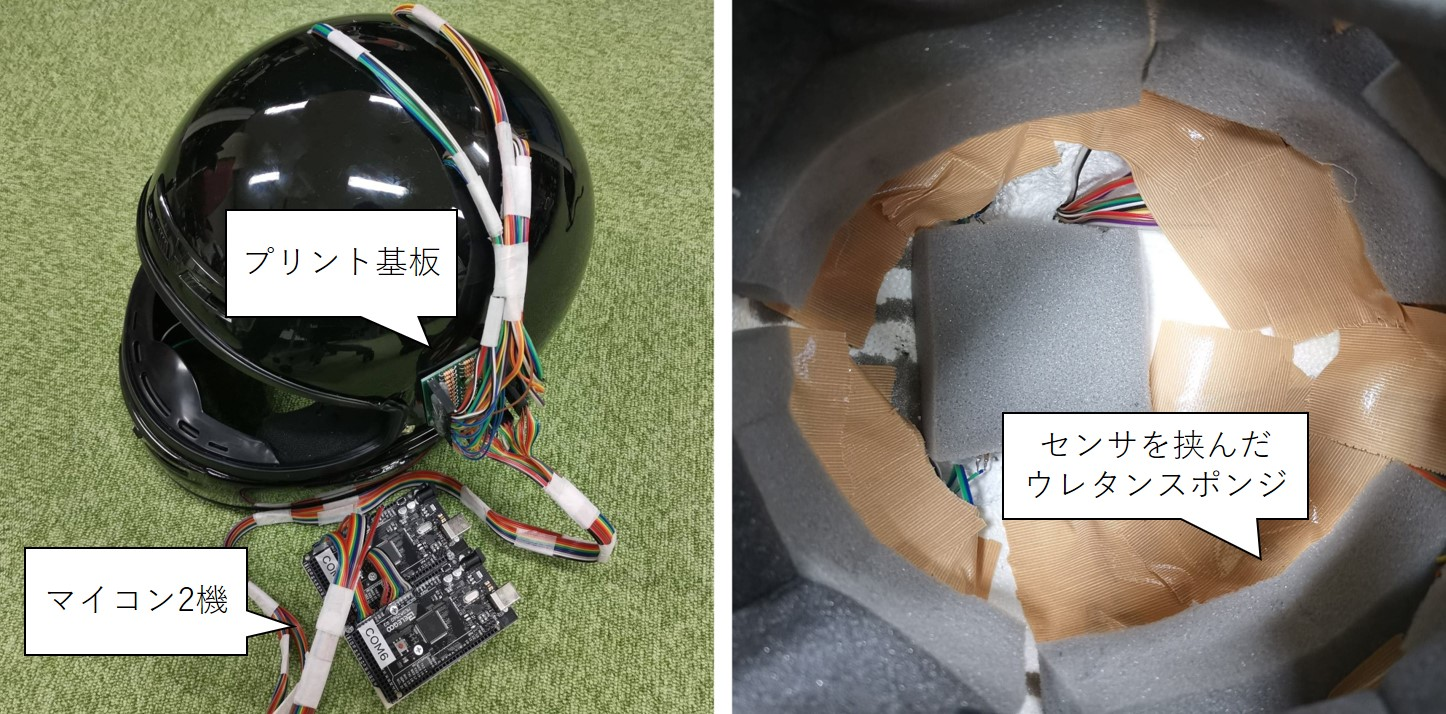
\includegraphics[width=1\linewidth]{met.eps}
  \end{center}
    \vspace{-8mm}
  \caption{実装したプロトタイプデバイス}
  \label{device}
\end{figure}

\begin{figure}[!t]
  \begin{center}
    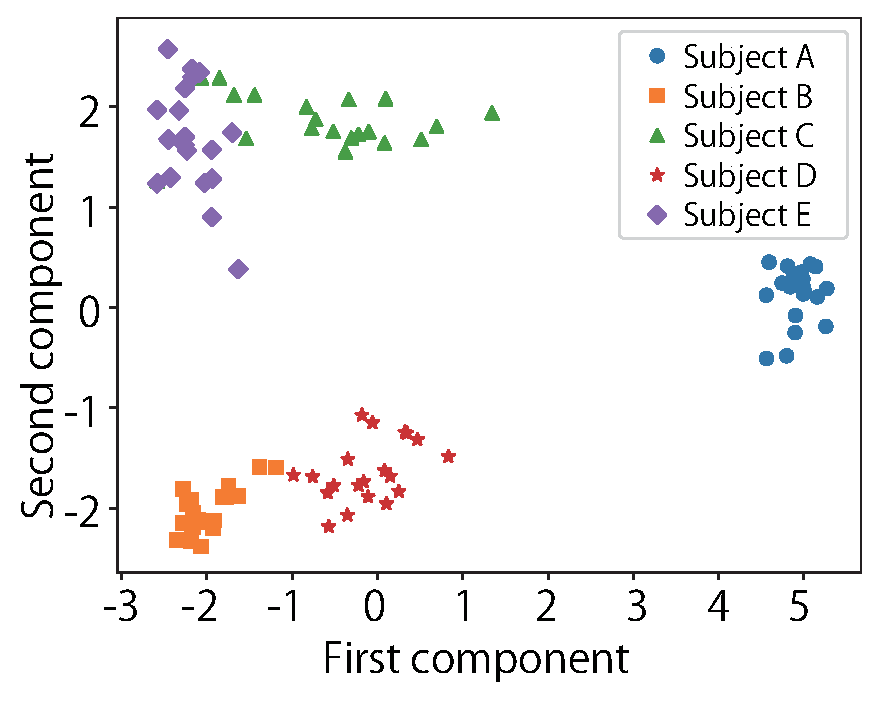
\includegraphics[width=1\linewidth]{PCA.eps}
  \end{center}
    \vspace{-8mm}
  \caption{PCAによる分析結果}
  \label{pca}
\end{figure}

%\bibliography{references}
%\bibliographystyle{junsrt}

%\begin{thebibliography}{2}
 %\bibitem{bib1} 白川功浩,吉浦 裕,市野将嗣:虹彩および目の周辺の分割画像を用いた個人認証,情報処理学会論文誌,Vol. 59,No. 9,pp. 1726--1738 (2018).
%\bibitem{bib2} 新島有信,伊勢崎隆司,青木良輔,渡部智樹,山田智広:導電性高分子電極を用いた帽子型筋電センサの提案,電子情報通信学会論文誌D,Vol. J101-D,No. 10,pp. 1378-1387 (2018).
% \end{thebibliography}
%\end{document}
